\documentclass[tikz,border=6pt]{standalone}
\usepackage{tikz}
\usetikzlibrary{calc}

\begin{document}
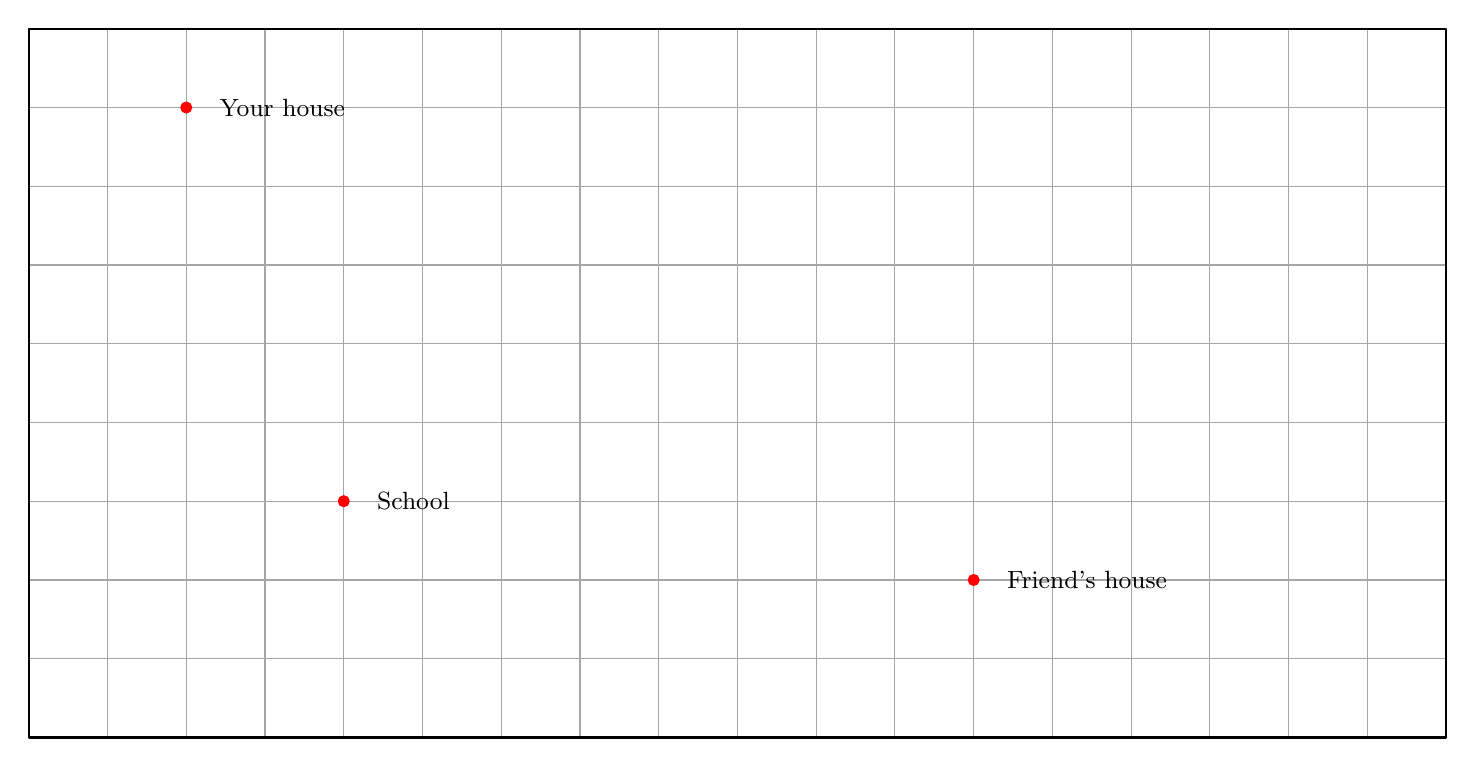
\begin{tikzpicture}[x=1cm,y=1cm, line cap=round, line join=round, font=\small]

% =========================================================
% A) THAM SỐ (chỉ chỉnh ở đây)
% =========================================================
% Lưới
\def\xMin{0}
\def\xMax{18}
\def\yMin{0}
\def\yMax{9}

% Tọa độ 3 điểm (chọn để giống bố cục hình mẫu)
\coordinate (H) at (2,8);     % Your house
\coordinate (S) at (4,3);     % School
\coordinate (F) at (12,2);  % Friend's house

% Kiểu điểm
\tikzset{
  gridline/.style={draw=black!35, line width=0.4pt},
  border/.style={draw=black, line width=0.8pt},
  dot/.style={circle, fill=red, draw=red, inner sep=1.4pt}
}

% =========================================================
% B) VẼ LƯỚI + KHUNG
% =========================================================
\draw[gridline] (\xMin,\yMin) grid (\xMax,\yMax);
\draw[border] (\xMin,\yMin) rectangle (\xMax,\yMax);

% =========================================================
% C) ĐIỂM + NHÃN
% =========================================================
\node[dot] at (H) {};
\node[dot] at (S) {};
\node[dot] at (F) {};

\node[anchor=west] at ($(H)+(0.3,0)$) {Your house};
\node[anchor=west] at ($(S)+(0.3,0)$) {School};
\node[anchor=west] at ($(F)+(0.3,0)$) {Friend's house};

\end{tikzpicture}
\end{document}
